\documentclass{beamer}
\usepackage{beamerthemesplit}
\usepackage{graphics}
%\usepackage[lined,boxed]{algorithm2e}
\usepackage[lined,noend]{algorithm2e}
\usepackage{amsmath}
\usepackage{amssymb}
\usepackage{listings}
\usepackage{soul}
\usepackage{mathtools}
\usepackage{colortbl}

\makeatletter
\newcolumntype{W}{!{\smash{\vrule
\@width 4\arrayrulewidth
\@height\dimexpr\ht\@arstrutbox+2pt\relax
\@depth\dimexpr\dp\@arstrutbox+2pt\relax}}}
\makeatother
\definecolor{gray}{rgb}{.7,.7,.7}



\DeclarePairedDelimiter\ceil{\lceil}{\rceil}
\DeclarePairedDelimiter\floor{\lfloor}{\rfloor}

\lstset{
basicstyle=\small,
keywordstyle=\color{blue}\bfseries,
numbers=left,
numberstyle=\tiny,
numbersep=5pt,
showstringspaces=false,
showspaces=false,
captionpos=b,
frame=tb,
float=tbh,
,escapeinside={*@}{@*}
}
\usetheme{Boadilla}
\title{ Analysis of Algorithms}
\subtitle{Divide and Conquer Strategy}
\author{Hikmat Farhat}
%\email{hfarhat@ndu.edu.lb}
%\institution{Notre Dame University}
\newtheorem{mydef}{Definition}
\newtheorem{lem}{Lemma}
%\newcommand{\emphasis}[1]{\textcolor{yellow}{#1}}
%\newcommand{\emphasis}[1]{\hl{#1}}
\newcommand{\emphasis}[1]{\ul{#1}}
%\newcommand{\floor}[1]{\lfloor{#1}\rfloor}
%\newcommand{\bfloor}[1]{\Big\lfloor{#1}\Big\rfloor}

%\newcommand{\gets}[0]{\leftarrow}

%\newcommand{\gets}{\ensuremath{\leftarrow}}
%\DeclareTextFontCommand{\emph}{\emphasis}
\sethlcolor{yellow}
\begin{document}

% title page
\frame{\titlepage}

\section{Binary Search}
\begin{frame}
  \frametitle{Binary Search}
  \begin{itemize}
  \item The simplest example of divide-and-conquer strategy is probably binary search.
\item Given a \textbf{sorted} array $A$ of $n$ elements and a value $x$, return \textbf{true} if $x$ is an element of $A$.
\item The key in this problem is that $A$ is \textbf{sorted}.
\item We follow a divide-and-conquer strategy by considering the "middle" element $m$ of $A$, and considering the half of $A$ to the left of $m$, $L$,
and the other half to the right of $m$, $R$.
\item Since $A$ is sorted then all elements of $L$ are less or equal than $m$ and all elements of $R$ are greater or equal than $m$.
  \end{itemize}
\end{frame}

\begin{frame}[fragile]
  \frametitle{Binary Search Code}
\begin{lstlisting}
bool binarySearch(int *A,int l,int r,int x){
   int m=(l+r)/2;

   if(x==A[m])return true;
   if(x>A[m]) 
      return binarySearch(A,m+1,r,x);
   else 
      return binarySearch(A,l,m-1,x);
}
\end{lstlisting}
  \begin{itemize}
  \item The complexity of the above code obeys the recurrence 
    \begin{align*}
      T(n)=T(\frac{n}{2})+\Theta(1)
    \end{align*}
\item The solution of the recurrence (see Master theorem later) is $T(n)=\Theta(\log n)$.
  \end{itemize}
\end{frame}


\section{Counting Inversions}


\begin{frame}[fragile]

\frametitle{Counting Inversions}
  \begin{itemize}
  \item Given an array $A$, a pair of elements $(A[i],A[j])$ is said to be an inversion iff $i<j$ and $A[i]>A[j]$.
  \item The simplest way to count the number of inversions in an array is using a double loop
  \end{itemize}
\begin{lstlisting}
count=0;
for(int i=1;i<n;i++){
   for(int j=0;j<i-1;j++){
     if(A[i]<A[j])count++;
   }
}
\end{lstlisting}
  \begin{itemize}
  \item Obviously the above algorithm is $\Theta(n^2)$.
  \item We will use divide-and-conquer to count the inversions in $\Theta(n\log n)$.
  \end{itemize}
\end{frame}
\begin{frame}
  \frametitle{Modified Merge Sort}
  \begin{center}
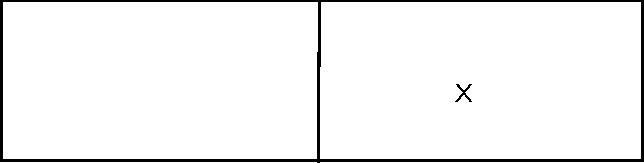
\includegraphics[width=0.5\textwidth]{divide-figs/inversions}    
  \end{center}

  \begin{itemize}
  \item If we divide an array in two then the total number of inversions is the sum of three parts
    \begin{enumerate}
    \item Inversions in the left part
    \item Inversions in the right part
    \item Inversions of elements of the right part relative to elements on the left part
    \end{enumerate}
\item The first two part are just recursive calls.
\item The third part can be computed using the merge procedure of merge sort
\item Note that in the above figure the inversions due to element $x$ relative to elements in the left part are the same whether the parts are sorted or not.
\end{itemize}
\end{frame}


\begin{frame}
  \begin{itemize}  \item The basic idea for the counting algorithm is to modify the merge procedure of merge sort to allow us to count the inversion.
  \item Given two sorted arrays $L$ and $R$, we merge them the same way as it was done using merge sort
\item Let $i$ and $j$ be the indices of elements of $L$ and $R$ respectively where initially $i=j=0$ we merge $L$ and $R$ into an array $C$ indexed
   by $k$.
 \item If $L[i]<R[j]$ then $L[i]$ is copied to $C[k]$ and $i=i+1$ and $k=k+1$.
 \item If $R[j]<L[i]$ then $R[j]$ is copied to $C[k]$ and $j=j+1$ and $k=k+1$. Also in this case all the remaining elements of $L$ are
larger than $R[j]$ which means that the number of inversions is incremented by the number of elements remaining in $L$.
\end{itemize}

\end{frame}

\begin{frame}
\frametitle{Example}
\begin{itemize}
\item  $L=\{\underset{\underset{i}{\uparrow}}{2},7,12\}$ and $R=\{\underset{\underset{j}{\uparrow}}{4},8,15\}$. 
\item First copy 2 to $C$ to obtain $L=\{2,\underset{\underset{i}{\uparrow}}{7},12\}$ and $R=\{\underset{\underset{j}{\uparrow}}{4},8,15\}$. 
\item Copy 4 to $C$ and increment the number of inversions by 2 because there are two elements remaining in $L$, namely 7 and 12. to obtain
\item  $L=\{2,\underset{\underset{i}{\uparrow}}{7},12\}$ and $R=\{4,\underset{\underset{j}{\uparrow}}{8},15\}$. 
\item Copy 7 to $C$ to obtain $L=\{2,7,\underset{\underset{i}{\uparrow}}{12}\}$ and $R=\{4,\underset{\underset{j}{\uparrow}}{8},15\}$. 
\item Copy 8 to $C$ and increment the number of inversions by 1 because there is one element remaining in $L$, namely 12.
\item The total number of inversions is 3.

  \end{itemize}
\end{frame}


\section{Master Theorem}
\begin{frame}
  \frametitle{Master Theorem (special case)}
  \begin{itemize}
  \item A generalization of the previous cases is done using a \textbf{simplified} version of the Master theorem
  \end{itemize}
  \begin{align*}
    T(n)=aT(n/b)+\Theta(n^d)
  \end{align*}
\end{frame}
\begin{frame}
  \begin{align*}
    T(n)&=aT(n/b)+cn^d\\
        &=a\left[aT(n/b^2)+c(n/b)^d\right]+cn^d\\
        &=a^2T(n/b^2)+cn^d(a/b^d)+cn^d\\
        &=a^2\left[aT(n/b^3)+c(n/b^2)^d\right]+cn^d(a/b^d)+cn^d\\
        &=a^3T(n/b^3)+cn^d(a/b^d)^2+cn^d(a/b^d)+cn^d\\
        &=a^iT(n/b^i)+cn^d\sum_{l=0}^{i-1}(a/b^d)^l
  \end{align*}
The above reaches $T(1)$ when $b^k=n$ for some $k$. We get
\end{frame}
\begin{frame}
    \begin{align*}
    T(n)&=a^kT(1)+cn^d\sum_{l=0}^{k-1}(a/b^d)^l
  \end{align*}
There are three cases
\begin{enumerate}
\item $a=b^d$
\item $a< b^d$
\item $a> b^d$
\end{enumerate}
\end{frame}
\begin{frame}
\frametitle{case 1: $a=b^d$}
 If $a=b^d$ (i.e $\frac{a}{b^d}=1$) then we get
 \begin{align*}
    T(n)&=a^kT(1)+cn^d\cdot k
  \end{align*}
Since $k=\log_b n$ then
 \begin{align*}
    T(n)&=a^{\log_bn}T(1)+cn^d\log_b n\\
        &=n^{\log_b a}T(1)+cn^d\log_bn\\
        &=n^dT(1)+cn^d\log_b n\\
        &=\Theta(n^d\log n)
  \end{align*}
\end{frame}
\begin{frame}
  \frametitle{case 2: $a<b^d$}
   \begin{align*}
    T(n)&=a^kT(1)+cn^d\sum_{l=0}^{k-1}(a/b^d)^l\\
        &=a^kT(1)+cn^d\frac{(a/b^d)^k-1}{(a/b^d)-1}
  \end{align*}
for large $n$, i.e. $n\rightarrow\infty$ then $k=\log_b
n\rightarrow\infty$ and since $a<b^d$ then $a/b^d\rightarrow 0$
Therefore
 \begin{align*}
    T(n)&=n^{\log_b a}T(1)+cn^d
  \end{align*}
but $a< b^d\Rightarrow \log_b a <d$ and finally
\begin{align*}
    T(n)&=\Theta(n^d)
  \end{align*}
\end{frame}
\begin{frame}
  \frametitle{case 3: $a>b^d$}
  In this case we can write
 \begin{align*}
    T(n)&=a^kT(1)+cn^d\frac{(a/b^d)^k-1}{(a/b^d)-1}\\
        &=n^{\log_b a}T(1)+gn^d(a/b^d)^k\\
        &=n^{\log_b a}T(1)+gn^d(a/b^d)^{log_b n}\\
        &=n^{\log_b a}T(1)+gn^dn^{log_b (a/b^d)}\\
        &=n^{\log_b a}T(1)+gn^dn^{(-d+log_b a)}\\
        &=\Theta(n^{\log_b a})
  \end{align*}
\end{frame}

\section{Maximum Subarray Sum}
\begin{frame}
  \frametitle{Maximum Subarray Sum}
  \begin{itemize}
  \item Given an array $A$ of $n$ elements we ask for the maximum
    value of
    \begin{align*}
 \sum_{k=i}^{j}A_k
    \end{align*}

\item For example if $A$ is -2,11,-4,13,-5,-2 then the answer is  $20=\sum_{k=2}^4$
  \end{itemize}
\end{frame}

\begin{frame}[fragile,fragile]
  \frametitle{Brute Force}
  \begin{itemize}
  \item Compute the sum of all subarrays of an array $A$ of size $n$ and return the largest.
  \item A subarray starts at index $i$ and ends at index $j$ where
    $0\le i< n$ and $0\le j <n$.
\item Therefore for \textbf{each possible} $i$ and $j$ compute the sum
  of $A[i]\ldots A[j]$.
  \end{itemize}
\begin{lstlisting}[frame=none,numbers=none]
int maxSubarray(int *A,int n){
  int sum=0, max=A[0];

  for(int i=0;i<n;i++){
      for(j=i;j<n;j++){
          sum=0;
         for(int k=i;k<=j;k++)
             sum+=A[k];
        if(max<sum)max=sum;
      }
  }
return max;
}
\end{lstlisting}
\end{frame}


\begin{frame}
  \frametitle{Complexity}
  \begin{itemize}
  \item To determine the complexity of the brute force approach we can
    see that there are 3 nested loop therefore the complexity of the
    problem depends on how many times line 14 is executed
\item The number of executions is
  \begin{align*}
    \sum_{i=0}^{n-1}\sum_{j=i}^{n-1}\sum_{k=i}^{j}1&=\sum_{i=0}^{n-1}\sum_{j=i}^{n-1}j-i+1\\
  \end{align*}
\item To evaluate the first sum let $m=j-i+1$ then
  \begin{align*}
    \sum_{j=i}^{n-1}j-i+1=\sum_{m=1}^{n-i}m=(n-i)(n-i+1)/2
  \end{align*}
  \end{itemize}
\end{frame}

\begin{frame}
  \begin{itemize}
  \item Finally, we get
 \begin{align*}
    \sum_{i=0}^{n-1}(n-i)(n-i+1)/2 &=\frac{n^3+3n^2+2n}{6}\\
   &=\Theta(n^3)
  \end{align*}
  \end{itemize}
\end{frame}

\begin{frame}
  \frametitle{Divide and Conquer}
  \begin{itemize}
  \item general technique that divides a problem in 2 or more parts (divide) and
    patch the subproblems together (conquer).
  \item In this context if we divide an array in two subarrays. We
    have  3    possibilities:
    \begin{enumerate}
    \item max is entirely in the first half
    \item max is entirely in the second half
     \item max spans both halves.
    \end{enumerate}
\item Therefore the solution is max(left,right,both)
  \end{itemize}
\end{frame}

\begin{frame}
  \frametitle{Both halves}
  \begin{itemize}
  \item If the sum spans both halves it means it includes the last
    element of the first half and the first element of the second half
\item This means that the we are looking for the sum of
  \begin{enumerate}
  \item Max subsequence in first half that includes the last element
  \item Max subsequence in the second half that includes the first element
  \end{enumerate}
  \end{itemize}
  \begin{align*}
    S_3&=\max_{\substack{0\le i< n/2\\n/2\le j<n}}\sum_{k=i}^jA[k]\\
      &=\max_{\substack{0\le i<
          n/2\\n/2\le j<n}}\left[\sum_{k=i}^{n/2-1}A[k]+\sum_{k=n/2}^jA[k]\right]\\
      &=\max_{0\le i< n/2}\sum_{k=i}^{n/2-1}A[k]+\max_{n/2\le j<n}\sum_{k=n/2}^jA[k]\\
  \end{align*}
\end{frame}
\begin{frame}
  \frametitle{Computing max that spans both halves}
   \begin{function}[H]
 
  \DontPrintSemicolon
  \SetKwFunction{computeBoth}{computeBoth}
\computeBoth(A,left,right)
\BlankLine
  $sum_1\gets sum_2\gets 0$\;
  $center\gets (left+right)/2$\;
 \For{$i=center$ \KwTo $left$}{
    $sum_1\gets sum_1+A[i]$\;
    \If{$sum_1>max_1$}{$max_1\gets sum_1$\;}
  }
 \For{$j=center+1$ \KwTo $right$}{
    $sum_2\gets sum_2+A[j]$\;
    \If{$sum_2>max_2$}{$max_2\gets sum_2$\;}
  }
\Return $max_1+max_2$\;
\end{function}
\end{frame}
\begin{frame}
  \frametitle{Recursive Algorithm}
  \begin{function}[H]
 
  \DontPrintSemicolon
  \SetKwFunction{maxSubarray}{maxSubarray}
  \maxSubarray{$A,left,right$}
  \BlankLine
  \If{$left=right$}{
   \Return $A[left]$
  }
  $center\gets (left+right)/2$\;
  $S_1\gets \maxSubarray(A,left,center)$\;
  $S_2\gets \maxSubarray(A,center+1,right)$\;
  $S_3\gets computeBoth(A,left,right)$\;
  \Return max($S_1,S_2,S_3$)\;
\end{function}
\end{frame}

% \begin{frame}
%   \frametitle{Implementation}
%   \begin{figure}[h]
%     \centering
% \lstset{basicstyle=\small}
% \lstset{basicstyle=\tiny}
% \lstinputlisting[frame=tbrl,linerange={6-29},name=class,caption={divide-and-conquer},label={lst:subsequence}]{divide-figs/subsequence.cpp}  
    
%   \end{figure}
% \end{frame}

% \begin{frame}
%   \frametitle{Implementation}
%   \begin{figure}[h]
%     \centering
% \lstset{basicstyle=\small}
% \lstset{basicstyle=\tiny}
%     \lstinputlisting[frame=tbr,linerange={30-50},name=class,caption={divide-and-conquer},label={lst:subsequence}]{divide-figs/subsequence.cpp}  
    
%   \end{figure}
% \end{frame}

\begin{frame}
  \frametitle{Complexity}
  \begin{itemize}
  \item Given an array of size $n$ the cost of the call to $maxSubarray$ is
    divided into two computations
    \begin{enumerate}
  \item The work of $computeBoth$ which is $\Theta(n)$.
  \item \textbf{Two} recursive calls on the problem with \textbf{half the size}
  \item Therefore the total cost can be written as
    \begin{align*}
      T(n)=2T(n/2)+\Theta(n)
    \end{align*}
    \end{enumerate}
\item Using the Master theorem we get $T(n)=\Theta(n\log n)$
  \end{itemize}
\end{frame}



\section{Medians}

\begin{frame}
  \frametitle{Medians}
  \begin{itemize}
  \item The \textit{median},$m$ of a sequence of $n$ numbers is defined such that half of values (more precisely $\floor*{n/2}$) of the sequence are bigger than $m$. For example
  for the sequence $48,5,10,25,42$ the median is 25.
  \item Obviously the median of $n$ numbers can be computed by sorting the sequence in $\Theta(n\log n)$ steps then selecting the value at position $\floor*{n/2}$
  \item Can we do better?
  \item It turns out that yes, by solving the general problem of selecting the $k^{\text{th}}$ smallest element of an array of $n$ elements.
  \end{itemize}
\end{frame}

\begin{frame}
  \frametitle{Strategy}
  \begin{itemize}
  \item We use a divide and conquer strategy as follows:
    \begin{enumerate}
    \item Given an array $A$ of $n$ elements, select \textit{randomly} a value $m$ from $A$.
    \item Partition $A$ into three arrays: $L$ that contains all the elements smaller than $m$ in no particular order, $E$ all the elements
    that are equal to $m$ and $R$ an array containing all the elements bigger than $m$.
  \item Now we have three cases:
    \begin{enumerate}
   \item if $k\le \mid L\mid $ then the $k^{\text{th}}$ element is in $L$ and we call the algorithm recursively on the, smaller array, $L$
    \item if $\mid L\mid < k\le \mid L\mid +\mid E\mid$ then the $k^{\text{th}}$ element is in $E$ and therefore it is equal to $m$.
  \item  if $m > \mid L\mid +\mid E\mid $ then the $k^{\text{th}}$ element is in $R$ and we call the algorithm recursively on the, smaller array, $R$
    \end{enumerate}
    \end{enumerate}
  \end{itemize}
\end{frame}

\begin{frame}
    \begin{function}[H]
 
  \DontPrintSemicolon
  \SetKwFunction{Select}{Select}
\SetKwFunction{Partition}{Partition}
  \Select{$A,left,right,k$}
  \BlankLine
  \If{$left=right$}{\Return $A[left]$\;}
  $m\gets random(left,right)$\;
  $val\gets A[m]$\;
  \Partition{$A,L,E,R,m$}\;
  \If{ $k\le\mid L\mid$ }{
    \Return \Select{$A,left,left+\mid L\mid -1,k$}\;
}
 \ElseIf{ $\mid L\mid <k\le \mid E\mid+\mid L\mid$}{
   \Return val\;
}
\Else{
\Return \Select{$A,left+\mid E\mid+\mid L\mid ,right,k-\mid E\mid-\mid L\mid$}\;
}
 
\end{function}
\end{frame}

% \begin{frame}
%   \frametitle{Example}
%   \begin{itemize}
%   \item As an example let us compute the $6^{\text{th}}$ smallest element in  the array $A=5,8,12,2,28,15,12,20$
% \item Assume that the selected element is 12
%   \end{itemize}
% \end{frame}

\begin{frame}
  \frametitle{The partition algorithm}
  \begin{itemize}
  \item The partition algorithm is a simple extension of the partition algorithm used for quicksort.
  \item In the select algorithm we had the arrays in the order $L$, $E$, $R$.
\item for convenience and similar to the partition in quicksort the partitions will look like the figure below
  \end{itemize}
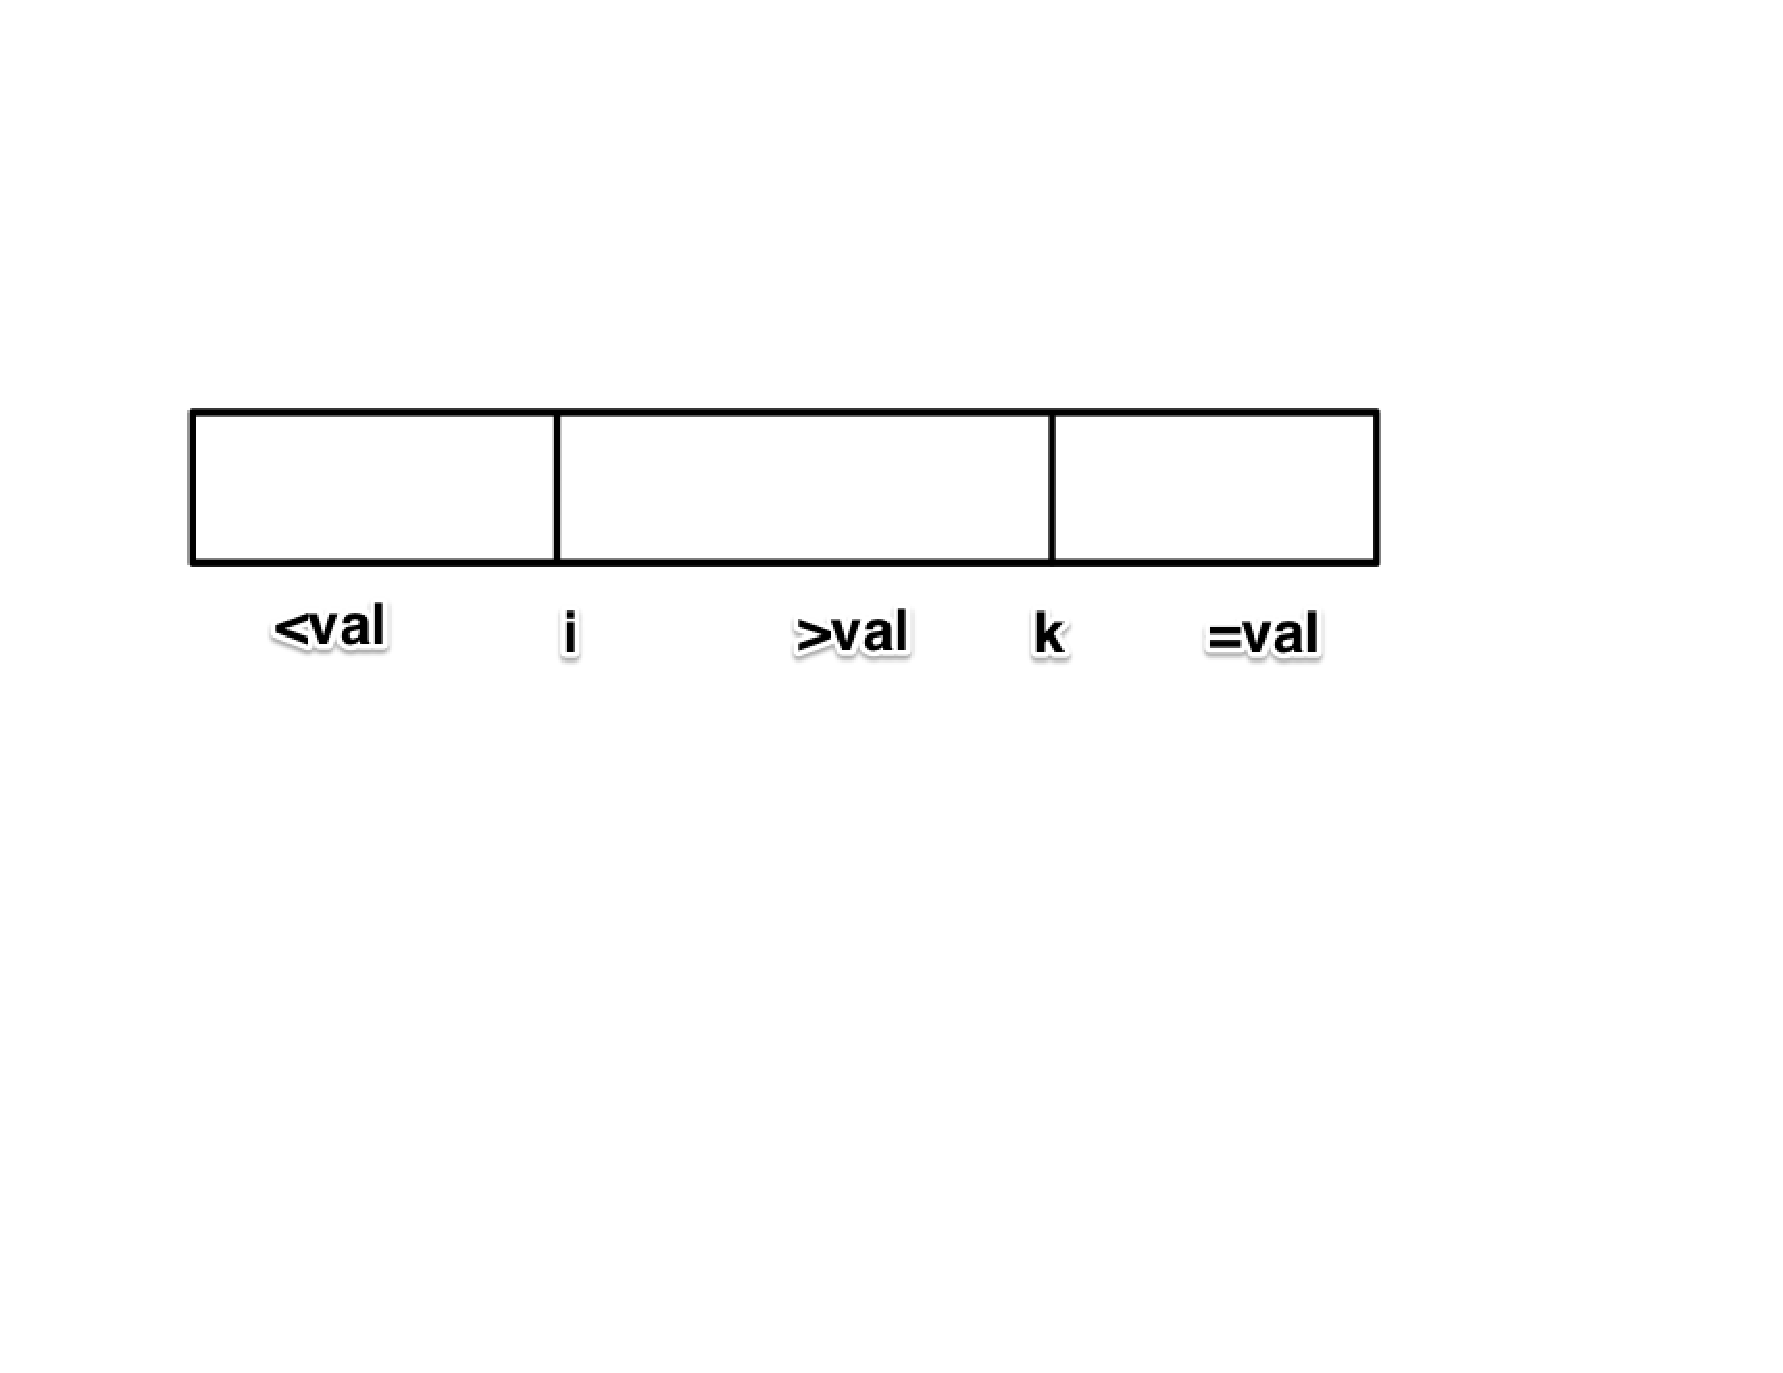
\includegraphics[width=0.9\textwidth]{divide-figs/partition}

\end{frame}


\begin{frame}
  \frametitle{Partitioning Algorithm}
  \begin{itemize}
  \item Assuming that the pivot is already in place in $a[r]$.
  \end{itemize}
\small{
  \begin{algorithm}[H]
\SetKwFunction{KwFn}{PARTITION(a,p,r)}
\DontPrintSemicolon
%\dontprintsemicolon
\KwFn \;
$i\gets p-1$\;
$k\gets p$\;
$j\gets r$\;
$pivot\gets a[r]$\;
\While{$k<j$}{
  \uIf{$a[k]> pivot$}{
   $k\gets k+1$\;
  }
  \uElseIf{$a[k]<pivot$} {
   $i\gets i+1$\;
   swap($a[i],a[k]$)\;
   $k\gets k+1$\;
  }
\Else{
$j\gets j-1$\;
swap($a[j],a[k]$)\;
}
}
\Return $i,j$
  \end{algorithm}
}
\end{frame}

\begin{frame}
  \begin{itemize}
  \item The partition algorithm is used by the select algorithm as follows:
    \begin{itemize}
    \item the array $L$ is $a[p]\ldots a[i]$.
    \item the array $E$ is $a[j]\ldots a[r]$.
    \item the array $R$ is $a[i+1]\ldots a[j-1]$.
    \item In code for the select algorithm we assumed that the order of the subarrays is $L$ followed by $E$ followed by $R$.
   \item Using the partitioning we modified select is 
    \end{itemize}
  \end{itemize}
\end{frame}




\begin{frame}
  \begin{function}[H]
 
  \DontPrintSemicolon
  \SetKwFunction{Select}{Select}
\SetKwFunction{Partition}{Partition}
  \Select{$A,left,right,k$}
  \BlankLine
  \If{left==right}{
    \Return A[left]\;
  }
  $m\gets random(left,right)$\;
  $val\gets A[m]$\;
  \Partition{$A,i,j,m$}\;
  \If{ $k\le i-left+1$ }{
    \Return \Select{$A,left,i,k$}\;
}
 \ElseIf{ $k\le i-s+e-j+2$}{
   \Return val\;
}
\Else{
\Return \Select{$A,i+1 ,j-1,k-(right-left+i-j+2)$}\;
}
 
\end{function}  
\end{frame}
\begin{frame}

\begin{itemize}
	\item the complexity of the k selection problem depends on both the recursive part and the partition part. 
	\item for an array of $n$ items the partition part is clearly $\Theta(n)$.
	\item The recursive part depends on the pivot. Suppose the pivot is the $i^{\text{th}}$ element then the subproblems are of size $i$ (i.e. from 0 to $i-1$) and $n-i-1$ (i.e from $i+1$ and $n-1$)
	\item In the k selection problem, unlike quicksort, the recursion is called on only one subproblem.
	\item the worst case behavior occurs when the algorithm repeatedly selects the largest or the smallest element as the pivot.
	\item in this case the subproblem size is $n-1$ and the algorithm obeys the recurrence
	\begin{displaymath}
		T(n)=T(n-1)+\Theta(n)
	\end{displaymath}
	\item whose solution is $T(n)=\Theta(n^2)$
\end{itemize}	
\end{frame}


\begin{frame}
	\frametitle{Average case complexity}
	
	\begin{itemize}
		\item The average case complexity is much better than the worst case
		\item we start by assuming that any index can be equally likely selected as the pivot
		\item Since the algorithm selects only one subproblem we can bound the complexity by selecting the largest subproblem. Let $X_i$ be a random variable

	\begin{displaymath}
		T(n)=T(max(i,n-i-1))+\Theta(n)
	\end{displaymath}
	\item averaging over all possible values of $i$ we get
	\begin{align*}
		T(n)&=\frac{1}{n}\sum_{i=0}^{n-1}T(max(i,n-i-1))+\Theta(n)\\
		    &=\frac{2}{n}\sum_{i=\lfloor n/2\rfloor}^{n-1}T(i)+\Theta(n)
	\end{align*}
	
	\end{itemize}
	
\end{frame}

\begin{frame}
we use the substitution method to prove that the average case complexity is $O(n)$. To show that $T(n)=O(n)$ we need to find $c>0$ and $n_0$ such that $T(n)\le c n$ for all $n\ge n_0$.

% \begin{itemize}
% \item Assuming that $T(n)$ is a nondecreasing function then $T(1)\le T(2)\le \ldots \le T(n_0-1)=d$ then we can write
% \begin{align*}
% T(n_0)&=\frac{2}{n_0}\sum_{k=\lfloor n_0/2\rfloor}^{n_0-1}T(k)	+O(n_0)\\
% &\le d +a\cdot n_0
% \end{align*}
% \item if we choose $c$ such that $c> d+a$ then $T(n_0)\le c\cdot n_0$
% \item This will be our base case for the induction.
\begin{itemize}
\item Now assume that $T(k)\le c\cdot k$ then the recurrence becomes
\begin{align*}
T(n)\le\frac{2}{n}\sum_{k=\lfloor n/2\rfloor}^{n-1}c\cdot k+a\cdot n	
\end{align*}

	
\end{itemize}

\end{frame}

\begin{frame}
  \begin{itemize}
  \item Keeping mind that $\floor{n/2}\ge n/2-1$
  \end{itemize}
\begin{align*}
T(n)&\le \frac{2\cdot c}{n}	\left( \sum_{k=0}^{n-1}k-\sum_{k=0}^{\lfloor n/2\rfloor -1}\right)k+a\cdot n &\\
&\le \frac{2\cdot c}{n}\left[ n(n-1)/2-\lfloor n/2\rfloor(\lfloor n/2\rfloor -1)/2\right]+a\cdot n &\\
&\le \frac{2\cdot c}{n}\left[ n(n-1)/2-(n/2-1)(n/2-2)/2\right]+a\cdot n &\\
&\le \frac{c}{n}\left[n^2-n-n^2/4+3n/2-2     \right]+a\cdot n&\\
&\le \frac{c}{n} (3n^2/4+n/2-2)+ a\cdot n &\\
&\le c\cdot n-\left(\frac{c\cdot n}{4}-\frac{c}{2}-a\cdot n \right) &
\end{align*}
\begin{itemize}
\item choose $c>4a$ and $n_0=\frac{2c}{c-4a}$
\end{itemize}
\end{frame}

\section{Multiplication}
\begin{frame}
  \frametitle{Multiplying two numbers}
  \begin{itemize}
  \item Given 2 n-bit numbers the "traditional" multiplication takes $\Theta(n^2)$ since there are $n^2$ 2-bit multiplications and $\Theta(n)$ additions of $n-bit$ numbers (for a total of $\Theta(n^2)$.
\item In this section we give a divide-and-conquer algorithm to compute the product of two n-bit numbers.
\item The basic ideas is that an $n-bit$ $x$ can be divided into the most significant $n/2$ bits and least significant $n/2$ bit. Two numbers $x$ and $y$ can be written  as $x=x_1\cdot 2^{n/2}+x_0$ and $y=y_1\cdot 2^{n/2}+y_0$.
  \end{itemize}
\end{frame}

\begin{frame}
    \begin{figure}[h]
    \centering
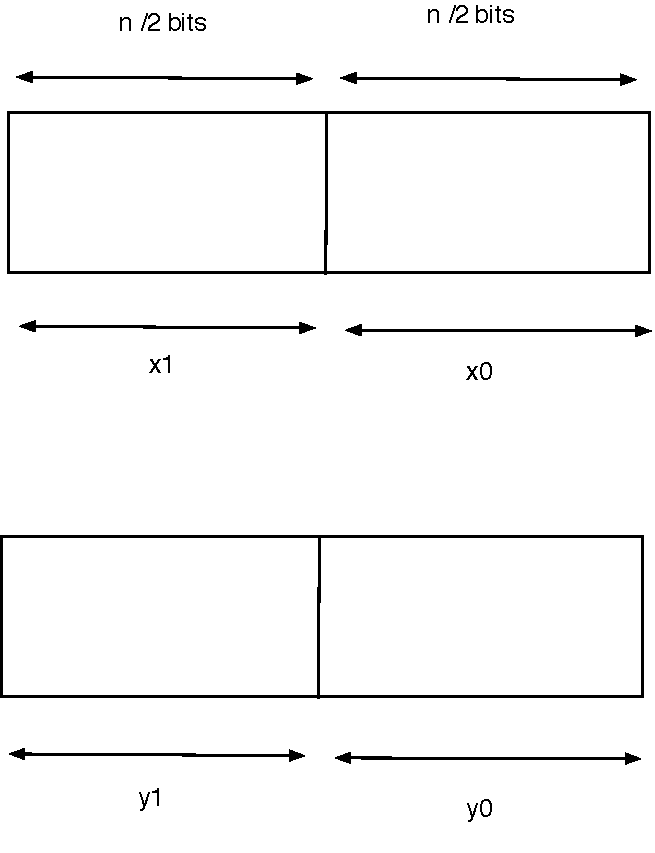
\includegraphics[width=0.5\textwidth]{divide-figs/multiplication}
  \end{figure}

\end{frame}
\begin{frame}
  \begin{itemize}
  \item Therefore $x\cdot y$ can be written as
    \begin{align*}
      &(x1\cdot 2^{n/2}+x0)\cdot(y1\cdot 2^{n/2}+y0)=\\
      &x1\cdot y1 \cdot 2^n+\\
      &(x1\cdot y0+x0\cdot y1)\cdot 2^{n/2}+x0\cdot y0
    \end{align*}
\item We have reduced the multiplication of $n$-bit numbers to that of $n/2$-bit numbers and multiplication by $2^n$ and $2^{n/2}$.
\item Multiplication by $2^n$ is equivalent with $n$-bit left shift and it can be done in $\Theta(n)$.
\item Therefore the recurrence can be written as

  \begin{align*}
    T(n)=4T(n/2)+\Theta(n)
  \end{align*}
\item Using the master theorem : $a=4,b=2,d=1$ The solution is $T(n)=\Theta(n^{\log_24})=\Theta(n^2)$ !!!
  \end{itemize}
\end{frame}
\begin{frame}
  \begin{itemize}
  \item We can get a better performance by noticing the following
    \begin{align*}
      (x1+x0)\cdot (y1+y0)=x1\cdot y1+x0\cdot y0+(x1\cdot y0+x0\cdot y1)
    \end{align*}
\item Rearranging terms we get
  \begin{align*}
(x1\cdot y0+x0\cdot y1)=(x1+x0)\cdot (y1+y0)-x1\cdot y1-x0\cdot y0
  \end{align*}
\item Since $x1\cdot y1$ and $x0\cdot y0$ are already computed then we need one extra multiplication instead of two. The recurrence becomes
  \begin{align*}
    T(n)=3T(n/2)+\Theta(n)
  \end{align*}
\item Thus $T(n)=\Theta(n^{\log_23})=\Theta(n^{1.58})$
  \end{itemize}
\end{frame}
\begin{frame}[fragile]
  \frametitle{Divide-and-Conquer algorithm}
\begin{lstlisting}
int multiply(int x,int y,int n){
  int x1=x>>n/2;
  int y1=y>>n/2;
  int mask=(1<<n/2)-1;
  int x0=x & mask;
  int y0=y &mask;
  int x1y1=multiply(x1,y1,n/2);
  int x0y0=multiply(x0,y0,n/2);
  int sum=x1y1+x0y0-multiply((x0+x1),(y0+y1),n/2);
  x1y1=x1y1<<n;
  sum=sum<<n/2;
  return x1y1+sum+x0y0;
}
\end{lstlisting}

\end{frame}

\section{Tower of Hanoi}

\begin{frame}[fragile]
  \frametitle{Tower of Hanoi}
  \begin{itemize}
  \item Let $move(n,start,end,aux)$ be the function that moves $n$ bricks from peg \textbf{start} to peg \textbf{end} using peg \textbf{aux} as auxiliary.
  \item Suppose that we can move $n-1$ bricks from the \textbf{start} peg and put them in \textbf{ aux} then all we have to do is move the remaining brick from \textbf{ start}
 to \textbf{end}\textbf{ then } transfer the $n-1$ from \textbf{ aux} to \textbf{ end}
\item we can write
  \end{itemize}
\begin{lstlisting}
move(n,start,end,aux){
 if(n==1)cout<<"("<<start<<","<<end<<")"<<endl;
 else { 
    move(n-1,start,aux,end);
    move(1,start,end,aux);
    move(n-1,aux,end,start);
 } 
\end{lstlisting}
\end{frame}
\begin{frame}
  \frametitle{Complexity}
  \begin{itemize}
  \item The solution to the Tower of Hanoi obeys the following recurrence relation
  \end{itemize}
    \begin{align*}
      T(n)&=2T(n-1)+\Theta(1)\\
          &=2T(n-1)+c\\
          &=2\left[2T(n-2)+c \right]+c\\
          &=2^2T(n-2)+2c+c\\
          &=2^2\left[2T(n-3)+c \right]+2c+c\\
          &=2^3T(n-3)+2^2c+2^1c+2^0c\\
          &\ldots\ldots\\
          &=2^kT(n-k)+\sum_{i=0}^{k-1}2^ic\\
          &=2^kT(n-k)+(2^k-1)c\\
    \end{align*}

\end{frame}
\begin{frame}
  \begin{itemize}
  \item The recursion stops when $k=n-1$ and we get
    \begin{align*}
      T(n)=2^{n-1}T(1)+(2^{n-1}-1)c=\Theta(2^n)
    \end{align*}
  \end{itemize}
\end{frame}
\end{document}

%%% Local Variables: 
%%% mode: late
%%% TeX-master: t
%%%
